\documentclass[11pt]{article}

\newcommand\reviewerVersion[2]{#1} % for review
%\newcommand\reviewerVersion[2]{#2} % separated tables and figures for production

\usepackage{amsmath, amssymb, amscd,amsthm}
\usepackage{color,graphicx} 

\newcommand\secWeakConvergence{S1}
\newcommand\secIIS{S2}
\newcommand\secGaussianIIS{S3}
\newcommand\secConjugacy{S4}
\newcommand\secPMCMC{S5}
\newcommand\SupSecLW{S6}
\newcommand\SupSecESS{S7}
\newcommand\SupSecBiBii{S8}
\newcommand\SupSecThmDetails{S9}

\usepackage{url} 
\newcommand\pomp{{\texttt{pomp}}}
\usepackage{verbatim}
\newcommand{\bbOmega}{\Omega}
\newcommand{\bbTheta}{\Theta}

\newcommand\IF{IF2}
\newcommand\IIS{IIS2}

\newcommand\asp{\hspace{4mm}}

\newcommand\Msigma{M}
\usepackage{amsmath,amssymb,thumbpdf}

\newcommand{\conditionList}{ %\setlength{\leftmargin}{0.2cm} 
\setlength{\topsep}{1mm} \setlength{\itemsep}{0.5mm} \setlength{\parsep}{0cm}}

\newcommand\HBf{\tilde f}
\newcommand\timeset{{\mathbb{T}}}
\newcommand\fzero{f}
\newcommand\Di{D1}
\newcommand\Dii{D2}
\newcommand\Diii{D3}
\newcommand\F{\mathcal{F}}
\newcommand\Amat{\Gamma}
\newcommand\Bmat{\Delta}
\newcommand{\hd}{\hat{\Delta}}
\newcommand{\bm}{\mbox{\boldmath{$\mu$}}}
\newcommand{\mc}{\mathcal}
\newcommand\resample[1]{K_{#1}}
\newcommand\extended{m}
\newcommand\ups{\upsilon}
\newcommand\mytheta{\theta}
\newcommand\Pspace{\mathbb{A}}
\newcommand\prob{\mathbb{P}}
\newcommand\E{\mathbb{E}}
\def\Var{\mathrm{Var}}
\def\var{\mathrm{Var}}
\def\Cov{\mathrm{Cov}} 
\def\R{\mathbb{R}}
\newcommand\lik{\ell}
\newcommand\Xspace{{\mathbb X}}
\newcommand\Yspace{{\mathbb Y}}
\newcommand\Thetaspace{{\bbTheta}}
\newcommand\hatTheta{\widehat{\Theta}}
%\newcommand\Thetaspace{{\mathbb T}}
\newcommand\Xdim{{\mathrm{dim}}(\Xspace)}
\newcommand\Ydim{{\mathrm{dim}}(\Yspace)}
\newcommand\Thetadim{{\mathrm{dim}}(\Thetaspace)}
\newcommand\ball{{\mathbb B}}
\newcommand\transpose{\prime}
\newcommand\given{{\, | \,}}
\newcommand\giventh{\,;}
\newcommand\mycolon{{\hspace{0.6mm}:\hspace{0.6mm}}}
\newcommand\normal{{\mathrm{Normal}}}

\newtheorem{prop}{Proposition}
\newtheorem{theorem}{Theorem}
\newtheorem{lemma}{Lemma}
\newtheorem{conjecture}{Conjecture}
 


\newcommand\listA{D}
\newcommand\listB{B}

\newcommand\Ca{C}
\newcommand\Cb{C_3}
\newcommand\Cc{C_4}

\newcommand\mZero{{m_0}} 
\newcommand\Disc{\mathrm{Disc}}

\usepackage{fullpage}
\renewcommand{\contentsname}{Supplementary Content}
\renewcommand{\refname}{Supplementary References}
\renewcommand\thefigure{S-\arabic{figure}}
\renewcommand\thetable{S-\arabic{table}}
\renewcommand\thepage{S-\arabic{page}}
\renewcommand\thesection{S\arabic{section}}
\renewcommand\theequation{S\arabic{equation}}
\renewcommand\thelemma{S\arabic{lemma}}
\renewcommand\thetheorem{S\arabic{theorem}}
\renewcommand\theprop{S\arabic{prop}}

\def\rmd{\mathrm{d}}
\newcommand{\eqdef}{\ensuremath{\stackrel{\mathrm{def}}{=}}}
\def\PE{\mathbb{E}} % esperance

\bibliographystyle{pnas2009}

\begin{document}
\begin{center}
{\bf \Large 
Supplement to ``Inference for dynamic and latent variable models via iterated, perturbed Bayes maps''
%Supplement to ``A new iterated filtering algorithm''
}
\end{center}
\bigskip
\begin{center}
\textbf{Edward L. Ionides$^1$, D. Nguyen$^1$, Y. Atchad\'{e}$^1$, S. Stoev$^1$ and A. A. King$^2$}
 
\vspace{3mm}
\today
\vspace{3mm}

{\small 
$^1$ Department of Statistics and $^2$Department of Ecology \& Evolutionary Biology,\\
The University of Michigan, Ann Arbor, Michigan, USA.  \\
email: ionides@umich.edu, nguyenxd@umich.edu, yvesa@umich.edu, sstoev@umich.edu, kingaa@umich.edu

\medskip

}
\end{center}

\vspace{4cm}


\tableofcontents

\newpage

\section{Weak convergence for occupation measures}
We study the convergence of the processes $\{W_\sigma(t),0\le t\le 1\}$ toward $\{W(t),0\le t\le 1\}$ as $\sigma\to 0$ for Theorem~2.
We are interested in showing that the fraction of time $\{W_\sigma(t)\}$ spends in a set $\Thetaspace_0\subset\Thetaspace$ over the discrete set of times $\{k\sigma^2,k=1,\dots,1/\sigma^2\}$ converges in distribution to the fraction of time $\{W(t)\}$ spends in  $\Thetaspace_0$.
We choose $\{W_\sigma(t)\}$ to be a right-continuous step function approximation to a diffusion to simplify the relationship between the occupancy fraction over the discrete set of times and over the continuous interval.
However, this simplification requires us to work with convergence to $\{W(t)\}$ in a space of processes with discontinuous sample paths, leading us to work with a Skorokhod topology.

Let $D_p[0,1]$ be the space of $\R^p$-valued functions on $[0,1]$ which are right-continuous with left limits.
Let $X= \{X(t)\}_{t\in [0,1]}$ and $\{X_n(t)\}_{t\in [0,1]}$, $n\ge 1$, be  stochastic processes with paths in $D_p[0,1]$. 
Let $\Rightarrow$ denote weak convergence, and suppose that $X_n\Rightarrow X$ as $n\to\infty$ in $D_p[0,1]$ equipped with the strong Skorokhod $J_1$ topology \cite{jacod87}.

\begin{prop}[Proposition VI.1.17 of \cite{jacod87}]
If $X$ has continuous paths, then $X_n \Rightarrow X$ as $n\to\infty$ in the space $D_p[0,1]$ equipped with the 
uniform metric. 
\end{prop}
Suppose that $f:\R^p \to \R$ is Borel measurable function and define the map $T_f:D_p[0,1]\to \R$
\begin{equation}\nonumber
 T_f(x) := \int_0^1 f(x(t))\, dt,\ \ x\in D_p[0,1].
\end{equation}
Now, let  $\Disc(T_f)$ denote the set of discontinuity points of $T_f$, let $C_p[0,1]$ be the space of $\R^p$-valued continuous functions on $[0,1]$, and write $\mathrm{Leb}$ for Lebesgue measure. 

\begin{prop} Suppose that $f$ is bounded. We have that
\begin{equation}\label{e:fact2}
\Disc (T_f) \cap C_p[0,1] \, \subset \, {\Big\{} x \in C[0,1]\, :\, {\rm Leb}(\{t\in [0,1]\, :\, x(t) \in \Disc(f) \})>0 {\Big\}} =:D_f.
\end{equation}
\end{prop}
\begin{proof}
Suppose that $x \in C_p[0,1]$ does not belong to the right--hand side of \eqref{e:fact2} and let
$x_n\to x$ in $J_1$. Then, according to a standard property of the Skorokhod $J_1$ topology \cite{jacod87}
we also have $\sup_{t\in [0,1]} |x_n(t) - x(t)| \to 0$, as $n\to\infty$. Now, since $x\not \in D_f$, we have that 
for almost all $t\in [0,1]$, the point $x(t)$ is a continuity point of $f$. Therefore, $f(x_n(t)) \to f(x(t)),\ n\to\infty$,
for almost all $t\in [0,1]$. Since $f$ is bounded, the Lebesgue dominated convergence theorem then yields
\begin{equation}\nonumber
T_f(x_n) \equiv  \int_0^1 f(x_n(t)) dt \longrightarrow \int_0^1 f(x(t))dt \equiv T_f(x),\ \ \mbox { as }n\to\infty.
\end{equation}
This completes the proof. 
\end{proof}
In the context of stochastic processes, by the Continuous Mapping Theorem, we have convergence in distribution,
\begin{equation*}
 T_f(X_n) \stackrel{d}{\longrightarrow} T_f(X),\ \ \mbox{ as }n\to\infty,
\end{equation*}
provided $X$ has continuous paths and $\prob (X \in \Disc(f))  = 0$. In the case when $f(x) = 1_A(x)$, the latter translates to
\begin{equation}\label{e:condition}
 \prob\{ \mbox{ The measure of the time $X$ spends on the boundary of $A$ is zero}\}  = 1.
\end{equation}
If the stochastic process has continuous marginal distribution and the set $A$ has zero boundary, the Fubini's theorem readily implies
\eqref{e:condition}. Indeed, the probability in \eqref{e:condition} equals
$$
\int_{\Omega}  \int_{0}^1 1_{\partial A}(X(t,\omega )) \, dt \, \prob(d\omega) = \int_0^1 \prob (X(t) \in \partial A) \, dt = 0, 
$$
provided that ${\rm Leb}(\partial A) =0$ and if $X(t)$ has a marginal density for each $t\in (0,1)$.
The above arguments lead to the proof of the following result.

\begin{lemma} Suppose that $X_n\Rightarrow X$ in $D_p[0,1]$, equipped with the uniform convergence topology.
If the process $X$ takes values in $C_p[0,1]$ and has continuous marginal distributions, then for all bounded Borel functions $f:\R^p \to \R$,
that are continuous almost everywhere, i.e.\ such that ${\rm Leb}(\Disc(f)) = 0$, we have
$$
\int_0^1 f(X_n(t)) \, dt \stackrel{d}{\longrightarrow} \int_0^1 f(X(t)) \, dt,\ \ \mbox{ as }n\to\infty.
$$
\end{lemma}

%%%%%%%%%%% GAUSSIAN %%%%%%%%%%%%%%%%%%%%%%%%%%%%%%%%%%

\section{Iterated importance sampling}

When $N=1$ in IF2, we obtain a general latent variable algorithm in which each iteration involves importance sampling but not filtering. 
This situation is called iterated importance sampling \cite{ionides11} and we call this special case of our algorithm IIS2.
Iterated importance sampling has previously been used to provide a route into proving convergence of iterated filtering \cite{ionides11,doucet13}.
However, in this article we found it more convenient to prove the full result for iterated filtering directly. 
Although IIS2 may have some independent value as a practical algorithm, our only use of IIS2 in this article is to provide a convenient environment for explicit computations for Gaussian models in Section~\ref{sec:gaussian} and non-Gaussian models in Section~\ref{sec:conjugate}.

\vspace{10mm}

\begin{center}
\noindent\begin{tabular}{l}
\hline
{\bf Algorithm~{\IIS}. Iterated importance sampling}\rule[-1.5mm]{0mm}{6mm}\\
\hline
{\bf input:}\rule[-1.5mm]{0mm}{6mm} \\
\begin{tabular}{ll}
Simulator for $f_{X}(x\giventh\theta)$ &
Evaluator for $f_{Y|X}(y\given x\giventh\theta)$\\
Data, $y^*$ &
Number of iterations, $M$ \\
Initial parameter swarm, $\{\Theta^0_j, \mbox{ $j$ in $1\mycolon J$}\}$ &
Number of particles, $J$ \\
Perturbation density, $h(\theta\given\varphi\giventh\sigma)$&
Perturbation sequence, $\sigma_{1:M}$ 
\end{tabular}\\
{\bf output:}\rule[-1.5mm]{0mm}{6mm} 
Final parameter swarm, $\{\Theta^M_j, \mbox{ $j$ in $1\mycolon J$}\}$ \\
For $m$ in $1\mycolon M$\rule[0mm]{0mm}{5mm}\\
\asp     $\Phi^{m}_{j}\sim h(\theta\given\Theta^{m-1}_{j}\giventh \sigma_m)$ for $j$ in $1\mycolon J$\\
\asp     $X_{j}^{m}\sim f_{X}(x\giventh \Phi^{m}_{j})$ for $j$ in $1\mycolon J$\\
\asp  $w_{j}^m = f_{Y|X}(y^*\given X_{j}^{m}\giventh \Phi^{m}_{j})$ for $j$ in $1\mycolon J$ \\
\asp  Draw $k_{1:J}$ with $\prob(k_j=i)=  w_{n,i}^m\Big/\sum_{u=1}^J w_{n,u}^m$  \\
\asp  $\Theta^{m}_{j}=\Phi^{m}_{k_j}$ for $j$ in $1\mycolon J$  \\
End For\\
\hline
\end{tabular}
\end{center}

\vspace{5mm}

A general latent variable model can be specified by a joint density $f_{XY}(x,y;\theta)$, with $X$ taking values in $\Xspace\subset \R^{\Xdim}$, $Y$ taking values in $\Yspace\subset \R^{\Ydim}$ and $\theta$ taking values in $\Thetaspace\subset\R^{\Thetadim}$. 
The data consist of a single observation, $y^*\in \Yspace$. 
The likelihood function is
\begin{equation}\nonumber
\lik(\theta)=f_Y(y^*;\theta)=\int f_{XY}(x,y^*;\theta)\, dx,
\end{equation}
and we look for a maximum likelihood estimate (MLE), i.e., a value $\hat\theta$ maximizing $\lik(\theta)$.
The parameter perturbation step of Algorithm~{\IIS} is a Monte~Carlo approximation to a perturbation map $H_{\sigma}$ where
\begin{equation}\label{eq:perturb_map}
H_\sigma g(\mytheta)=\int g(\varphi)h(\theta\given\varphi\giventh\sigma)\, d\varphi.
\end{equation}
A natural choice for $h(\,\cdot\,\given\varphi\giventh\sigma)$ is the multivariate normal density with mean $\varphi$ and variance $\sigma^2\Sigma$ for some covariance matrix $\Sigma$, but in general $h$ could be any condition density parameterized by $\sigma$.
The resampling step of Algorithm~{\IIS} is a Monte~Carlo approximation to a Bayes map, $B$, given by
\begin{equation}\label{eq:bayes_map}
Bf(\mytheta)=f(\mytheta)\lik(\mytheta)\Big\{\int f(\varphi)\lik(\varphi)\, d\varphi\Big\}^{-1}.
\end{equation}
When the standard deviation of the parameter perturbations is held fixed at $\sigma_m=\sigma>0$, Algorithm~{\IIS} is a Monte Carlo approximation to $T_\sigma^M\fzero(\theta)$ where
\begin{equation}
\label{recursion}
T_\sigma f(\mytheta) =  BH_\sigma f(\mytheta)= \frac{\int f(\varphi)\, \lik(\theta) h(\theta\given\varphi\giventh\sigma)\, d\varphi}{\int \!\! \int f(\varphi)\, \lik(\xi) h(\xi\given\varphi\giventh\sigma)\, d\varphi \, d\xi}.
\end{equation}

\section{Gaussian and near-Gaussian analysis of iterated importance sampling}\label{sec:gaussian}

The convergence results of Theorems~1 and~2 in the main text are not precise about the rate of convergence, either toward the MLE as $\sigma\to 0$ or toward the stationary distribution as $M\to\infty$. 
Explicit results are available in the Gaussian case and are also relevant to near-Gaussian situations.
The near-Gaussian situation may arise in practice, since the parameter perturbations can be constructed to follow a Gaussian distribution and the log likelihood surface may be approximately quadratic due to asymptotic behavior of the likelihood for large sample sizes.
The near-Gaussian situation for a POMP model does not require that the POMP itself is near Gaussian, only that the log likelihood surface is near quadratic.
Here, we consider only the univariate case, and only for iterated importance sampling. 
We offer this simplified case as an illustrative example, rather than an alternative justification for the use of our algorithm.
In principle, these results can be generalized, but such results do not add much to the general convergence guarantees already obtained.

We investigate the eigenvalues and eigenfunctions for a Gaussian system, and then we appeal to continuity of the eigenvalues to study systems that are close to Gaussian.
Here, we consider the case of a scalar parameter, $\dim(\Thetaspace=1)$, and an additive perturbation given by
\begin{equation}\label{eq:kappa}
h(\theta\given\varphi\giventh\sigma)= \kappa(\theta-\varphi).
\end{equation}
We first study the unnormalized version of (\ref{recursion}) defined as
\begin{equation}
\label{recursion:S}
Sf(\mytheta) = \big[ f(\mytheta)\, \lik(\mytheta) \big] * \kappa(\mytheta)
= \int\big[ f(\mytheta-\varphi)\, \lik(\mytheta-\varphi) \big] \, \kappa(\varphi)\, d\varphi.
\end{equation}
This is a linear map, and we obtain the eigenvalues and eigenfunctions when $\lik$ and $h$ are Gaussian in Proposition~\ref{prop:eigen}.
Iterations of the corresponding normalized map, $T_\sigma$, converge to the normalized eigenfunction corresponding to the largest eigenvalue of $S$, which can be seen by postponing normalization until having carried out a large number of iterations of the unnormalized map.
Suppose, without loss of generality, that the maximum of the likelihood is at $\theta=0$. 
Let $\phi(\mytheta;\sigma)$ be the normal density with mean zero and variance $\sigma^2$.
\begin{prop}\label{prop:eigen}
Let $S_0$ be the map constructed as in (\ref{recursion:S}) with the choices
$\lik(\mytheta)=\phi(\mytheta;\tau)$ and $\kappa(\mytheta)=\phi(\mytheta;\sigma)$. Let 
\begin{equation}
u^2 = \left(\sigma^2+\sqrt{\sigma^4+4\sigma^2\tau^2}\right)/2 = \sigma\tau + o(\sigma).
\end{equation}
The eigenvalues of $S_0$ are 
$$
\lambda_n = \sigma\tau \sqrt{2\pi}\left( \frac{u^2-\sigma^2}{u^2}\right)^{(n+1)/2},
$$
for $n=0,1,2,\dots$, and the corresponding eigenfunctions have the form
\begin{equation}
\label{eq:eigenFuncs}
e_n = p_n(\mytheta)\phi(\mytheta;u),
\end{equation}
where $p_n$ is a polynomial of degree $n$.
\end{prop}
\begin{proof}
Let $P_n$ be the subspace of functions of the form $q(\mytheta)\phi(\mytheta;u)$ where $q$ is a polynomial of degree less than or equal to $n$. We show that $S_0$ maps $P_n$ into itself, and look at what happens to terms of degree $n$.
Let $H_n$ be the Hermite polynomial of degree $n$, defined by $(d/d\mytheta)^n \phi(\mytheta;1)= (-1)^n H_n(\mytheta) \phi(\mytheta;1)$.
Let  $\alpha = (1/u^2 + 1/\tau^2)^{-1/2}$, and set
\begin{equation}\label{f}
f(\mytheta) = \alpha^{-2n} H_n(\mytheta/\alpha)\phi(\mytheta;u).
\end{equation}
Then,
\begin{equation}
f(\theta)\lik(\theta) = \frac{\alpha}{\sigma\tau \sqrt{2\pi}}\,  \alpha^{-2n} H_n(\mytheta/\alpha)\phi(\mytheta;\alpha) = \frac{\alpha}{\sigma\tau \sqrt{2\pi}} (-1)^n \frac{d^n}{d\mytheta^n} \phi(\mytheta;\alpha).
\end{equation}
Since $\big[(d/d\mytheta)^n f\lik\big] * \kappa = (d/d\mytheta)^n\big[(f\lik)*\kappa \big]$, we get
\begin{equation}\label{fg*h}
(f\lik)*\kappa = \frac{\alpha}{\sigma\tau \sqrt{2\pi}} (-1)^n \frac{d^n}{d\mytheta^n} \phi(\mytheta;u) = \frac{\alpha}{\sigma\tau \sqrt{2\pi}}
u^{-2n}H_n(\mytheta/u)\phi(\mytheta;u).
\end{equation}
Writing $H_n(\mytheta)=h_0+h_1\mytheta+\dots+h_n\mytheta^n$, we see that the coefficient of the term in $\mytheta^n$ in (\ref{f}) is $\alpha^{-n}h_n
$, whereas in (\ref{fg*h}) it is $\frac{\alpha}{\sigma\tau \sqrt{2\pi}}u^{-n}$.
We have shown that $S_0$ operating on $P_n$ multiplies the coefficient of degree $n$ by a factor of $\lambda_n$.
Letting $L_n$ be the matrix representing $S_0$ on $P_n$ with the basis $b_0,\dots,b_m$ given by 
$b_m(\mytheta)=\mytheta^m\phi(\mytheta;u)$, we see that $L_n$ is lower triangular with diagonal entries $\lambda_0,\dots,\lambda_n$.
Therefore, the eigenvalues are $\lambda_0,\dots,\lambda_n$, and the eigenfunction corresponding to $\lambda_m$ is in $P_m$.
\end{proof}
The case where $\log\lik(\theta)$ is close to quadratic is relevant due to asymptotic log quadratic properties of the likelihood function.
Choosing $\kappa(\theta)$ to be Gaussian, as in Proposition~\ref{prop:eigen}, we have the following approximation result. 

\begin{prop}\label{prop:cont}
Let $S_\epsilon$ be a map as in (\ref{recursion:S}), with $\lik$ satisfying $\sup_\mytheta|\lik(\mytheta)-\phi(\mytheta;\tau)|<\epsilon$ and $\kappa(\mytheta)=\phi(\mytheta;\sigma)$. 
For $\epsilon$ small, the largest eigenvalue of $S_\epsilon$ is close to $\lambda_0$ and the corresponding eigenfunction is close to $\phi(\mytheta;u)$.
\end{prop}
\begin{proof}
Write $\lik(\mytheta)=\phi(\mytheta;\tau)+\eta(\mytheta)$, with $\sup_\mytheta |\eta(\mytheta)|<\epsilon$. Then,
\begin{equation}
\label{Seps}
\| S_\epsilon f - S_0 f \| = \|(f\eta)*\kappa \| \le \| f\eta\| \le \epsilon \|f\|.
\end{equation}
Here, $\|\cdot\|$ is the $L^2$ norm of a function or the corresponding operator norm (largest absolute eigenvalue). 
Convolution with $\kappa$ is a contraction in $L^2$, which is apparent by taking Fourier transforms and making use of Parseval's relationship, since all frequencies are shrunk by multiplying with the Fourier transform of $\kappa$.
From \eqref{Seps}, we have $\|S_0-S_\epsilon \|<\epsilon$. 
This implies that $S_\epsilon$ has a largest eigenvalue $\mu_0$ with $|\mu_0-\lambda_0|<\epsilon$, based on the representation that
\begin{equation}
|\mu_0| = \| S\| = \sup_f \frac{\|S_\epsilon f \|}{\|f \|}.
\end{equation}
Writing the corresponding unit eigenfunction as $w_0$, we have
%=\sum_{i=1}^\infty \alpha_i e_i$, with $\{e_i\}$ from~\eqref{eq:eigenFuncs},
\begin{equation}
\label{w_0}
w_0 = (1/\mu_0) S_\epsilon w_0 = (1/\mu_0)[S_0 w_0 + \eta],
\end{equation}
where $\|\eta(\mytheta)\|<\epsilon$. Writing $w_0=\sum_{i=1}^\infty \alpha_i e_i$, in terms of $\{e_i\}$ from~\eqref{eq:eigenFuncs}, equation~\eqref{w_0} gives
\begin{equation}
\sum_{i=1}^\infty \alpha_i e_i = \sum_{i=1}^\infty \alpha_i\frac{\lambda_i}{\mu_0} e_i
+\eta = \sum_{i=1}^\infty \alpha_i\frac{\lambda_i}{\lambda_0} e_i
+ \tilde \eta,
\end{equation}
where $\|\tilde \eta\| < \epsilon(1+[\lambda_0(\lambda_0-\epsilon)]^{-1})$.
Comparing terms in $e_i$, we see that all terms $\alpha_1,\alpha_2,\dots$ must be of order $\epsilon$.
\end{proof}

\section{A class of exact non-Gaussian limits for iterated importance sampling}\label{sec:conjugate}

We look for exact solutions to the equation $Tf=f$ where $T=BH$, as specified in \eqref{recursion} with $h(\theta\given\varphi\giventh\sigma)= \kappa(\theta-\varphi)$.
This situation corresponds to iterated importance sampling with additive parameter perturbations that have no dependence on $\sigma$, as in equation~\eqref{eq:kappa}. 
Now, for $g(x)$ being a probability density on $\Thetaspace$, define
 \begin{equation} \label{eq:lik:conjugate}
 \lik_g(x) = c \frac{g(x)}{\kappa * g (x)},
\end{equation}
where $c$ is a non-negative constant. 
For likelihood functions of the form \eqref{eq:lik:conjugate}, supposing that $\lik_g$ is integrable, we obtain an eigenfunction $e(x)=\kappa*g(x)$ for the unnormalized map $S$ defined in \eqref{recursion:S} via the following calculation:
\begin{eqnarray}
Se(x)&=& c \int \frac{g(x-u)}{(g *\kappa)(x-u)} (g*\kappa)(x-u) \kappa(u)\, du \\
&=& c \int g(x-u) \kappa(u)\, du \\
&=& c \big[ g* \kappa(x) \big]\quad = \quad c \, e(x).
\end{eqnarray}
Under conditions such as Theorem~1, it follows that $\kappa*g$ is the unique eigenfunction for $T$, up to a scale factor, and that $\lim_{M\to\infty}T^Mf=e$.
We do not anticipate practical applications for the conjugacy relationship we have established between the pair $(\lik_g,\kappa)$ since we see no reason why the likelihood should have the form of \eqref{eq:lik:conjugate}. 
However, this situation does serve to identify a range of possible limiting behaviors for $T^M$.

\section{Applying PMCMC to the cholera model}

\begin{figure}
\begin{center}

%\includegraphics[width=6.5in]{cholera/p3-flux/pmcmc-varplot}

\reviewerVersion{
\vspace{-3mm}

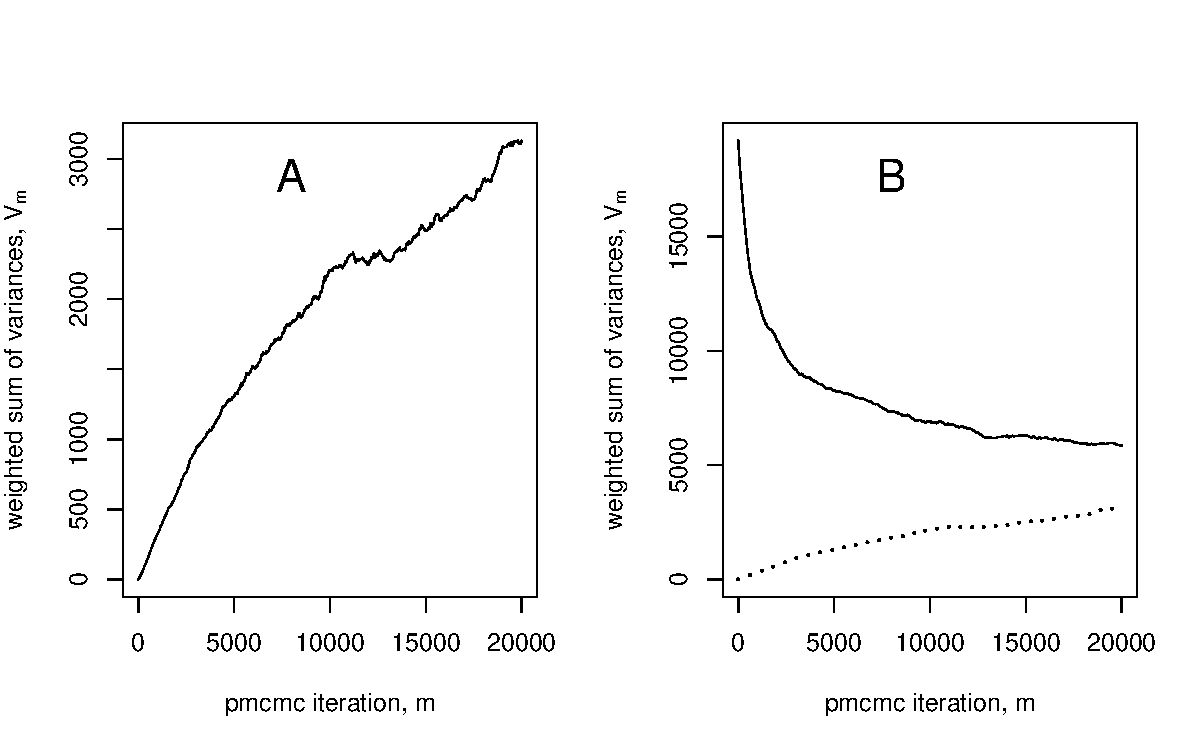
\includegraphics[width=6.5in]{figS1}

\vspace{-8mm}

}
{\medskip\texttt{Figure pdf in figS1.pdf. For review, please view supp-if2-review.pdf.}

\vspace{5mm}}


\end{center}
\caption{PMCMC convergence assessment, using the diagnostic quantity in equation~\ref{eq:pmcmc-Vm}. (A) Underdispersed chains, all started at the MLE. (B) Overdispersed chains, started with draws from the prior (solid line), and underdispersed chains (dotted line).
The average acceptance probability was $0.04238$, with Monte Carlo standard error $0.00072$, calculated from iterations 5000 through 20000 for the 100 underdispersed PMCMC chains.  For the overdispersed chains, the average acceptance probability was $0.04243$ with standard error $0.00100$.
}\label{fig:pmcmc-varplot}
\end{figure}

We carried out PMCMC for the cholera model, with the prior being uniform on the hyper-rectangle specified by $\theta_\mathrm{low}$ and $\theta_\mathrm{high}$ in Table~1.
Thus, the IF1 and IF2 searches were conducted starting with random draws from this prior.
Since PMCMC is known to be computationally demanding, we investigated a simplified challenge: investigating the posterior distribution starting at the MLE.
This would be appropriate, for example, if one aimed to obtain Bayesian inferences using PMCMC but giving it a helping hand by first finding a good starting value obtained by a maximization procedure.
We used the PMMH implementation of PMCMC in \texttt{pomp} \cite{pomp} with parameter proposals following a Gaussian random walk with standard deviations given by $(\theta_\mathrm{high}-\theta_\mathrm{low})/100$.
We started 100 independent chains at the estimated MLE in Table~1.
Each PMCMC chain, with $J=1500$ particles at each of $M=2\times10^4$ likelihood evaluations, took around 30 hours to run on a single core of the University of Michigan Flux cluster.
Writing $V_{m,d}$ for the sample variance of variable $d\in\{1,\dots,\Thetadim\}$ among the 100 chains at time $m\in\{1\dots,M\}$, and $\tau_d$ for the Gaussian random walk standard deviation for parameter $d$, we tracked the quantity
\begin{equation}\label{eq:pmcmc-Vm}
V_m=\sum_{d=1}^{\Thetadim} \frac{V_{m,d}}{\tau_d^{2}}.
\end{equation}
Supposing the posterior variance is finite, a necessary requirement for convergence to stationarity as $m$ increased is for $V_m$ to approach its asymptotic limit.
Since all the chains start at the same place, one expects $V_m$ to increase toward this limit. 
The number of iterations required for $V_m$ to stabilize therefore provides a lower bound on the time taken for convergence of the chain.
This test assesses the capability of the chain to explore the region of parameter space with high posterior probability density, rather than the capability to search for this region from a remote starting point.
We also tested PMCMC on a harder challenge, investigating convergence of the MCMC chain to its stationary distribution from over-dispersed starting values.
We repeated the computation described above, with 100 chains initialized at draws from the prior distribution.
The results are shown in Figure~\ref{fig:pmcmc-varplot}.
From Figure~\ref{fig:pmcmc-varplot}A, we see that the stationary distribution has not yet been approached for the chains starting at the MLE, since the variance of independent chains continues to increase up to $M=2\times 10^4$.
As a harder test, the variance for the initially overdispersed independent chains should approach that for the initially underdispersed chains, but we see in  Figure~\ref{fig:pmcmc-varplot}B that much more computation would be required to achieve this with the algorithmic settings used.

The PMCMC chains used here involved $JMN=(1.5\times 10^3)\times (2\times 10^4) \times (6\times 10^2)=1.8\times 10^{10}$ calls to the dynamic process simulator (the dominating computational expense), and yet failed to converge.
By contrast, IF2 with  $JMN=(10^4)\times 10^2 \times (6\times 10^2)=6\times 10^8$ calls to the dynamic process simulator was shown to be an effective tool for global investigation of the likelihood surface.
As with all numerical comparisons, it is hard to assess whether poor performance is a consequence of poor algorithmic choices. 
Conceptually, a major difference between iterated filtering and PMCMC is that the filtering particles in IF2 investigate the parameter space and latent dynamic variable space simultaneously, whereas in PMCMC each filtering iteration is used only to provide a single noisy likelihood evaluation.
It may not be surprising that algorithms such as PMCMC struggle in situations where filtering is a substantial computational expense and the likelihood surface is sufficiently complex that many thousands of Monte Carlo steps are required to explore it.
Indeed, IF1 and IF2 remain the only algorithms that have currently been demonstrated computationally capable of efficient likelihood-based inference for situations of comparable difficulty to our example.

\section{Applying Liu \& West's method to the toy example}

\begin{figure}
\begin{center}

%\includegraphics[width=6.5in]{toy/lw1/lw}

\reviewerVersion{
\vspace{-3mm}

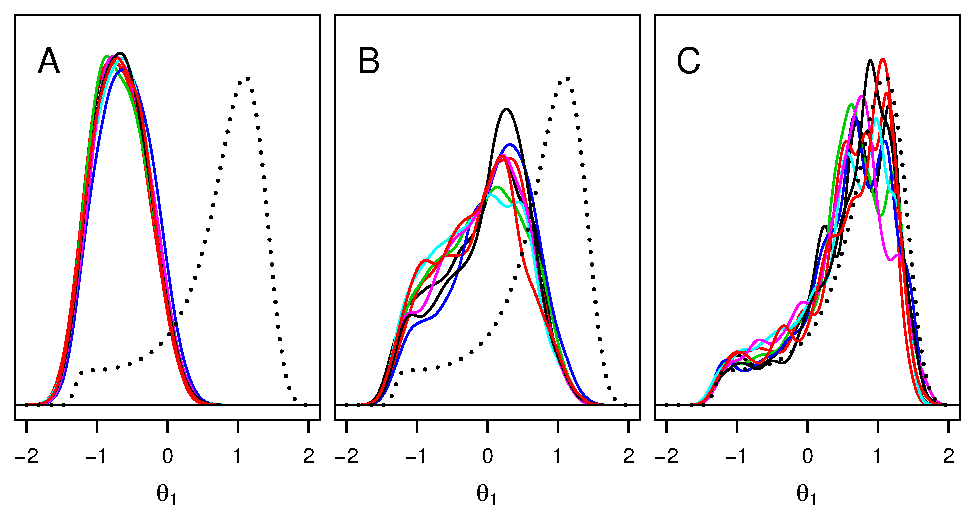
\includegraphics{figS2}

\vspace{-8mm}

}
{\medskip\texttt{Figure pdf in figS2.pdf. For review, please view supp-if2-review.pdf.}

\vspace{5mm}}  


\end{center}
\caption{The Liu \& West  algorithm \cite{janeliu01} applied to the toy example with varying values of the discount factor:
(A) $\delta=0.99$; (B) $\delta=0.999$; (C) $\delta=0.9999$.
Solid lines show 8 independent estimates of the marginal posterior density of $\theta_1$. The black dotted line shows the true posterior density.
}
\label{fig:sup:LW}
\end{figure}

Bayesian parameter estimation for POMP models using sequential Monte Carlo with perturbed parameters was proposed by \cite{kitagawa98}. 
Similar approaches using alternative nonlinear filters have also been widely used \cite{anderson79,wan00}.
Liu \& West \cite{janeliu01} proposed a development on the approach of \cite{kitagawa98} which combines parameter perturbations with a contraction that is designed to counterbalance the variation added by the perturbations, thereby approximating the posterior distribution of the parameters for the fixed parameter model of interest.
Liu \& West \cite{janeliu01} also included an auxiliary particle filter procedure  in their algorithm \cite{pitt99}.
The auxiliary particle filter is a version of sequential Monte Carlo which looks ahead to a future observation when deciding which particles to propagate.
Generally, auxiliary particle filter algorithms do not have the plug-and-play property \cite{breto09,he10} since they involve constructing weights that require evaluation of the transition density for the latent process.
In addition, the auxiliary particle filter does not necessarily have superior performance over a basic sequential Monte Carlo filter \cite{johansen08b}.
To compare with IF2 and PMCMC on our toy example, we therefore employ a version of the Liu \& West algorithm, which we call LW, that omits the auxiliary particle filter procedure.
LW carries out the key innovation of parameter perturbation and contraction (Steps 3 and 4 in Sec.~10.4 of \cite{janeliu01}) while omitting the auxiliary particle filter (Steps 1 and 2, and the denominator in Step~5, in Sec.~10.4 of \cite{janeliu01}).
LW was implemented via the \texttt{bsmc2} function of the \texttt{pomp} package \cite{pomp}.
If an effective auxiliary particle filter were available for a specific computation, it could also be used to enhance other sequential Monte Carlo based inference procedures such as IF1, IF2 and PMCMC.

For the numerical results reported in Fig.~\ref{fig:sup:LW} we used $J=10^4$ particles for LW.
This awards the same computational resources to LW that we gave IF1 and IF2 for the results in Fig.~1.
The magnitude of the perturbations in LW is controlled by a discount factor ($\delta$ in the notation of \cite{janeliu01}), and we considered three values, $\delta\in\{0.99,0.999,0.9999\}$.
Liu \& West \cite{janeliu01} suggested that $\delta$ should take values in the range $\delta\in[0.95,0.99]$, with smaller values of $\delta$ reducing Monte Carlo variability while increasing bias in the approximation to the target posterior distribution.
For our toy example, we see from Fig.~\ref{fig:sup:LW}A that the choice $\delta=0.99$ results in a stable Monte~Carlo computation (since all eight realizations are close).
However, Fig.~\ref{fig:sup:LW}A also reveals a large amount of bias.
Increasing $\delta$ to $0.999$, Fig.~\ref{fig:sup:LW}B shows some increase in the Monte~Carlo variability and some decrease in the bias.
Further increasing $\delta$ to $0.9999$, Fig.~\ref{fig:sup:LW}C shows the bias becomes small while the Monte~Carlo variability continues to increase.
Values of $\delta$ very close to one are numerically tractable for this toy model, but not in most applications. 
As $\delta$ approaches one, the ensuing numerical instability exemplifies the principal reason why Bayesian and likelihood-based inference for POMP models is challenging despite the development of modern nonlinear filtering techniques.

The justification provided by \cite{janeliu01} for their algorithm is based on a Gaussian approximation to the posterior distribution.
Specifically, \cite{janeliu01} argued that the posterior distribution should be approximately unchanged by carrying out a linear contraction toward its mean followed by adding an appropriate perturbation.
Therefore, it may be unsurprising that LW performs poorly in the presence of nonlinear ridges in the likelihood surface. 
Other authors have reported poor numerical performance for the  algorithm of \cite{janeliu01}, e.g., Fig.~2 of \cite{storvik02} and Fig.~2 of \cite{chopin13}. 
Our results are consistent with these findings, and we conclude that the approach of \cite{janeliu01} should be used with considerable caution when the posterior distribution is not close to Gaussian.


\section{Consequences of perturbing parameters for the numerical stability of SMC}

\begin{figure}


\begin{center}

%\includegraphics{cholera/f1/ess}

\reviewerVersion{
\vspace{-20mm}

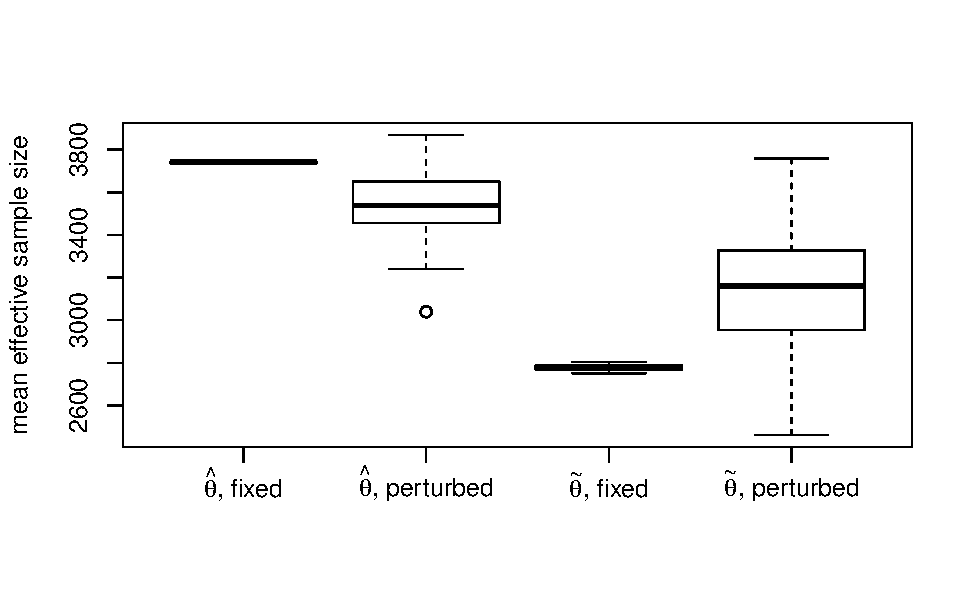
\includegraphics{figS3}

\vspace{-20mm}

}{\medskip\texttt{Figure pdf in figS3.pdf. For review, please view supp-if2-review.pdf.}}


\end{center}
\caption{Effective sample size (ESS) for SMC with fixed parameters and with perturbed parameters. 
We ran SMC for the cholera model with the parameter vector set at the MLE, $\hat\theta$, and at an alternative parameter vector $\tilde \theta$ for which the first 18 parameters in Table~1 were multiplied by a factor of 0.8. 
We defined the ESS at each time point by the reciprocal of the sum of squares of the normalized weights of the particles. The mean ESS was calculated as the average of these ESS values over the 600 time points. Repeating this computation 100 times, using $J=10^4$ particles, gave 100 mean ESS values shown in the ``fixed'' columns of the box-and-whisker plot. Repeating the computation with additional parameter perturbations having random walk standard deviation of 0.01 gave the 100 mean ESS values shown in the ``perturbed'' column. 
For both parameter vectors, the perturbations greatly increase the spread of the mean ESS.
At $\hat\theta$, the perturbations decreased the mean ESS value by 5\% on average, whereas at $\tilde\theta$ the perturbations increased the mean ESS value by 13\% on average.
The MLE may be expected to be a favorable parameter value for stable filtering, and our interpretation is that the parameter perturbations have some chance of moving the SMC particles away from this favorable region.
When started away from the MLE, the numerical stability of the IF2 algorithm benefits from the converse effect that the parameter perturbations will move the SMC particles preferentially toward this favorable region.
For parameter values even further  from the MLE than $\tilde\theta$, SMC may fail numerically for a fixed parameter value yet be feasible with perturbed parameters.
}\label{fig:ess}
\end{figure}


The IF2 algorithm applies sequential Monte Carlo (SMC) to an extended POMP model in which the time-varying parameters are treated as dynamic state variables.
This procedure increases the dimension of the state space by the number of time-varying parameters.
Empirically, SMC has been found effective in many low dimensional systems but its numerical performance can degrade in larger systems.
A natural concern, therefore, is the extent to which the extension of the state variable in IF2 increases the numerical challenge of carrying out SMC effectively. 
Two rival heuristics suggest different answers. 
One intuitive (but not universally correct) argument is that adding variability to the system stabilizes numerically unstable filtering problems, since it gives each particle at least a slim chance of following a trajectory compatible with the data.
An opposing intuition, that SMC breaks down rapidly as the dimension increases, has theoretical support \cite{bengtsson08}.
However, the theoretical arguments of \cite{bengtsson08} may be driven more by increasing the observation dimension than increasing the state dimension, so their relevance in the present situation is not entirely clear.

We investigated numerical stability of SMC, in the context of our cholera example, by measuring the effective sample size (ESS) \cite{liu01a}.
We investigated the ESS for two parameter vectors, the MLE and an alternative value for which SMC is more numerically challenging.
We carried out particle filtering with and without random walk perturbations to the parameters, obtaining the results presented in Fig.~\ref{fig:ess}.
We found that the random walk perturbations led to a 5\% decrease in the average ESS at the MLE, but a 13\% increase in the average ESS at the alternative parameter vector.
This example demonstrates that the random walk perturbations can have both a cost and a benefit for numerical stability, with the benefit outweighing the cost as the filtering problem becomes more challenging.



\section{Checking conditions B1 and B2}\label{sec:b1b2}

We check B1 and B2 when $\Theta$ is a rectangular region in $\R^{\Thetadim}$, with $h_n(\theta\given \phi\giventh\sigma)$ describing a Gaussian random walk having as a limit a reflected Brownian motion on $\Theta$. 
A more general study of the limit of reflected random walks to reflected Brownian motions (in particular, including limits where the random walk step distribution satisfies B5) was presented by Bossy et al.~\cite{bossy04}.
The specific examples of the IF2 algorithm given in our paper all employ Gaussian random walk perturbations for the parameters.
The examples did not employ boundary conditions to constrain the parameter to a bounded set. 
While such conditions could be used to ensure practical stability of the algorithm, we view the conditions primarily as a theoretical device to assist the mathematical analysis of the algorithm.

Suppose that $\Theta=[a_1,b_1]\times[a_2,b_2]\times...\times[a_{\Thetadim},b_{\Thetadim}]$. 
For each coordinate direction $d=1,\dots,\Thetadim$, let $R_d:\R\to[a_d,b_d]$ be the reflection map defined recursively by
\begin{equation*}
R_d(x)= \left\{
\begin{array}{lcl}
x &\mbox{if}& x\in[a_d,b_d]\\
R_d(2b_d-x)&\mbox{if}& x>b_d\\
R_d(2a_d-x)&\mbox{if}& x<a_d
\end{array}\right. .
\end{equation*}
Let $h_{n,d}(\theta_d\given \phi_d\giventh\sigma)$ be the density of
$R_d(\phi_d+\sigma Z)$ where $Z$ is a standard Normal random variable.
Let $h_n(\theta\given \phi\giventh\sigma)$ be the joint density corresponding to the product of $h_{n,1},\dots,h_{n,\Thetadim}$.
This choice of $h_n$ corresponds to a perturbation process for the parameter vector in the IF2 algorithm following a Gaussian random walk on $\Theta$ with reflective boundary conditions, independently in each coordinate direction. 
By construction, the finite dimensional distributions of $W_\sigma(t)$ at the set of times 
\begin{equation}\nonumber
\{k\sigma^2:k=0,1,2,\dots \mbox{ and } k\sigma^2\le 1\}
\end{equation}
 exactly match the corresponding finite dimensional distributions of a reflected Brownian motion $\{W(t)\}$ taking values in $\Theta$.
This $\{W(t)\}$ gives a construction of the limiting process whose existence is assumed in B1.
For $A\subset\Theta$, we see from this construction of $\{W(t)\}$ that the probability  $\{W(t)\}$ is in $A$ for all $\epsilon\le t\le 1]$ is greater than the corresponding probability for an unreflected Brownian motion, $\{W_{(u)}(t)\}$ with the same intensity parameter.
It is routine to check that $\{W_{(u)}(t)\}$ has a positive probability of remaining in any open set $A$ for all $\epsilon\le t\le 1$ uniformly over all values of $W_{(u)}(0)\in \Theta$.
Thus, we have completed the check of condition B1. 

To check B2,
%\eic{For B2, do we need an unbounded limit on $t$?}. 
the positivity of the marginal density of $W(t)$ on $\Theta$, uniformly over the value of $W(0)$, again follows since this density is larger than the known density for $W_{(u)}(t)$.


\section{Additional details for the proof of Theorem~1}

In the main text, a condensed proof of Theorem~1 is provided to describe the key steps in the argument. 
Here, we restate Theorem~1 and provide a more detailed proof.
The reader is referred back to the main text for the notation and statement of conditions B2 and B4. 

\medskip

\noindent {\bf Theorem 1}. 
{\it
Let $T_\sigma$ be the map defined by [1] in the main text, and suppose B2 and B4. There exists a unique probability density $f_\sigma$ such that for any probability density $f$ on $\Theta$,
\begin{equation}
\label{eq:sup:thm1.1}
\lim_{m\to\infty} \|T_\sigma^m f - f_\sigma\|_1=0,
\end{equation}
where $\|f\|_1$ is the $L^1$ norm of $f$.  Let $\{\Theta_j^M,\;j=1,\ldots,J\}$ be the output of IF2, with $\sigma_m=\sigma>0$. There exists a finite constant $\Ca$ such that 
\begin{equation}
\label{eq:sup:thm1.2}
\limsup_{M\to\infty}\mathbb{E}\left[\,\bigg|\,\frac{1}{J}\sum_{j=1}^J \phi(\Theta_j^M)- \int \phi(\theta)f_\sigma(\theta)\, d\theta\,\bigg|\,\right] \leq \frac{\Ca \sup_\theta|\phi(\theta)|}{\sqrt{J}}.
\end{equation}
}

\begin{proof}
Let $L^1(\Theta)$ denote the space of integrable real-valued functions on $\Theta$ with norm $\|f\|_1=\int|f(\theta)|\, d\theta$. 
For non-negative measures $\mu$ and $\nu$ on $\Theta$, let $\|\mu-\nu\|_{\textsf{tv}}$  denote the total variation distance and let $H(\mu,\nu)$ denote the Hilbert metric distance \cite{eveson95,legland04}.  
The measures $\mu$ and $\nu$ are said to be comparable if they are both nonzero and there exist constants $0<a\le b$ such that $a\,\nu(A)\le \mu(A)\le b\,\nu(A)$ for all measurable subsets $A\subset\Theta$. 
For comparable measures, $H(\mu,\nu)$ is defined by
\begin{equation}
H(\mu,\nu)=\log\frac{ \sup_A \mu(A)/\nu(A)}{ \inf_A \mu(A)/\nu(A)},
\end{equation}
with the supremum and infimum taken over measurable subsets $A\subset\Theta$ having $\nu(A)>0$. 
For noncomparable measures, the Hilbert metric is defined by $H(0,0)=0$ and otherwise $H(\mu,\nu)=\infty$.
The Hilbert metric is invariant to multiplication by a positive scalar, $H(a\mu,\nu)=H(\mu,\nu)$. 
This projective property makes the Hilbert metric convenient to investigate the Bayes map: in the context of the following proof, the projective property lets us analyze the linear map $S_\sigma$ to study the nonlinear map $T_\sigma$.
%\input{hilbert}

For $\theta_{0:N}\in \Theta^{N+1}$, we single out the last component of $\theta_{0:N}$ by writing  $\breve\ell(\theta_{0:N})= \breve\ell(\theta_{0:N-1},\theta_N)$ and  $h(\theta_{0:N}\given \phi)=h(\theta_{0:N-1},\theta_N\given \phi)$. Then, for $\phi$ and $\theta$ in $\Theta$, we define 
\begin{equation} \label{eq:sup:s}
s_\sigma(\phi,\theta)=\int h(\theta_{0:N-1},\theta\vert \phi,\sigma)\breve \ell(\theta_{0:N-1},\theta)\, d\theta_{0:N-1}.
\end{equation}
 The function $s_\sigma$ in \eqref{eq:sup:s} defines a linear operator $S_\sigma f(\theta)=\int s_\sigma(\phi,\theta) f(\phi)\rmd \phi$ that maps $L^1(\Theta)$ into itself. 
Notice that  $T_\sigma f(\theta) =S_\sigma f(\theta)/\| S_\sigma f\|_1$. 
More generally, if $\mu$ is a probability measure on $\Theta$, $S_\sigma \mu$ denotes  the function $S_\sigma\mu(\theta)=\int s_\sigma(\phi,\theta)\mu(d\phi)$. 
Notice also that $S_\sigma^m f$, the $m$-th iterate of $S_\sigma$, can be written as $S_\sigma^m f(\theta)=\int s^{(m)}_\sigma(\phi,\theta) f(\phi)d\phi$, where $s^{(1)}_\sigma(\phi,\theta) =s_\sigma(\phi,\theta)$, and for $m\geq 2$, $s^{(m)}_\sigma(\phi,\theta) =\int s_\sigma(\phi,u) s^{(m-1)}_\sigma(u,\theta) du$. 
Using the definition of $\breve\ell$ and B4,
\begin{eqnarray} \nonumber
s_\sigma(\phi,\theta)&=& \int h(\theta_{0:N-1},\theta\vert \phi,\sigma)\int f_X(x_{0:N}\vert \theta_{0:N-1},\theta)f_{Y\vert X}(y^*_{1:N}\vert x_{0:N})\, d x_{0:N}\, d \theta_{0:N-1}\\
&\geq& 
\label{eq:sup:s2}
\epsilon^N \int h(\theta_{0:N-1},\theta\vert \phi,\sigma)\, d \theta_{0:N-1},
\\
\nonumber
\mbox{\hspace{-6.5mm}and, similarly,}\hspace{6.5mm}&&
\\
\label{eq:sup:s3}
s_\sigma(\phi,\theta)&\leq& \epsilon^{-N}\int h(\theta_{0:N-1},\theta\vert \phi,\sigma)\, d \theta_{0:N-1}.
\end{eqnarray}
By iterating the inequalities \eqref{eq:sup:s2} and  \eqref{eq:sup:s3}, assumption B2 implies that there exists $\mZero\geq 1$ such that for any $m\geq \mZero$, there exist $0<\delta_{m}<\infty$, a probability measure $\lambda_m $ on $\Theta$ such that for all measurable subsets $A\subset\Theta$ and all $\theta\in\Theta$,
\begin{equation}\label{mixing}
\delta_{m}\lambda_m(A)\leq \int _A s^{(m)}(\theta,\phi)\, d \phi \leq \delta_{m}^{-1}\lambda_m(A).\end{equation}
 In other words, $S_\sigma^{\mZero}$ is mixing in the sense of \cite{legland04}. In the terminology of \cite{eveson95}, this means that for each $m\geq \mZero$, $S^m$ has finite projective diameter (see Lemma 2.6.2 of \cite{eveson95}). Therefore, by Theorem 2.5.1 of \cite{eveson95}, we conclude that $S_\sigma$  has a unique non-negative eigenfunction $f_\sigma$ with $\|f_\sigma\|_1=1$, and for any density $f$ on $\Theta$, as $q\to\infty$,
\[\left\|\frac{[S_\sigma^{\mZero}]^qf}{\|[S_\sigma^{\mZero}]^qf\|_1}-f_\sigma\right\|_1=\left\|T_\sigma^{{\mZero}q}f -f_\sigma\right\|_1\to 0.\]
This implies the statement \eqref{eq:sup:thm1.1}, by writing for any $m\geq 1$, $m=q \mZero +r$, for $0\leq r\leq \mZero-1$, and $T_\sigma^m f=[T_\sigma^{q\mZero}]T_\sigma^rf$.

Let the initial particle swarm $\{\Theta^0_j,\;1\leq j\leq J\}$ consist of independent draws from the density $f$.
To prove \eqref{eq:sup:thm1.2}, we decompose $M=q\mZero +r$, for some $r\in\{0,\ldots,\mZero-1\}$, and we introduce the empirical measures $\mu^{(0)}= J^{-1}\sum_{j=1}^J\delta_{\Theta_j^{(r)}}$, and for $k=1,\ldots,q$, $\mu^{(k)}= J^{-1}\sum_{j=1}^J\delta_{\Theta_j^{(r+{\mZero}k)}}$, so that $\mu^{(q)}=J^{-1}\sum_{j=1}^J\delta_{\Theta_j^{(M)}}$. We then write, for any bounded measurable function $\phi$,
\begin{eqnarray*}
\mu^{(q)}(\phi)-[T_\sigma^Mf](\phi)&=&\mu^{(q)}(\phi)-\left[T_\sigma^{{\mZero}q}\mu^{(0)}\right](\phi) + \left[T_\sigma^{{\mZero}q}\mu^{(0)}\right](\phi) -\Big[T_\sigma^{{\mZero}q}T_\sigma^{r}f\Big](\phi)\\
&=&\sum_{i=1}^q\bigg\{\Big[T_\sigma^{{\mZero}(i-1)}\mu^{(q-i+1)}\Big](\phi)-\Big[ T_\sigma^{{\mZero}i}\mu^{(q-i)}\Big](\phi)\bigg\}
\\
& & \hspace{2cm}+ \hspace{1mm}\left[T_\sigma^{{\mZero}q}\mu^{(0)}\right](\phi) -\Big[T_\sigma^{{\mZero}q}T_\sigma^{r}f\Big](\phi).
\end{eqnarray*} 
Using Theorem 2 of \cite{crisan02}, we can find a finite constant $\Cb$ such that for all $k\geq 1$,
 and writing $\|\phi\|_\infty=\sup_\theta|\phi(\theta)|$,
\begin{equation}\label{SMC:control}
\rho=\sup_{\phi:\;\|\phi\|_\infty=1 } \mathbb{E}\bigg[\left|\mu^{(k)}(\phi)-\big[T_\sigma^{{\mZero}}\mu^{(k-1)}\big](\phi)\right|\bigg] 
\; \leq \;
\frac{\Cb}{\sqrt{J}},
\end{equation}
with B4 implying that the constant $\Cb$ constructed by \cite{crisan02} does not depend on $\mu^{(k-1)}$.
Since $S_\sigma^{{\mZero}}$ is mixing and (\ref{mixing})  holds, using Lemma 3.4, Lemma 3.5, Lemma 3.8 and Equation (7) of \cite{legland04}, we have
\begin{eqnarray*}
\PE\bigg[\,\Big|\big[T_\sigma^{{\mZero}q}\mu^{(0)}\big](\phi) -\big[T_\sigma^{{\mZero}q}T_\sigma^{r}f\big](\phi)\Big|\,\bigg] 
&\leq & \|\phi\|_\infty \PE\bigg[\,\big\|T_\sigma^{{\mZero}q}\mu^{(0)} - T_\sigma^{{\mZero}q}T_\sigma^{r}f\big\|_{\textsf{tv}}\bigg]\\
& \leq & \frac{2\|\phi\|_\infty}{\log 3}\PE\left[H\left(S_\sigma^{{\mZero}q}\mu^{(0)}, S_\sigma^{{\mZero}q}T_\sigma^rf\right)\right]\\
&\leq& \frac{2\|\phi\|_\infty}{\log 3}\left(\frac{1-\delta^2_{{\mZero}}}{1+\delta^2_{{\mZero}}}\right)^{q-2}\frac{1}{\delta_{{\mZero}}^2}\PE\Big[\,\big\|T_\sigma^{{\mZero}}\mu^{(0)}- T_\sigma^{{\mZero}}T_\sigma^rf\big\|_{\textsf{tv}}\,\Big]\\
&\leq& \frac{4\|\phi\|_\infty}{\log 3}\left(\frac{1-\delta^2_{{\mZero}}}{1+\delta^2_{{\mZero}}}\right)^{q-2}\frac{1}{\delta_{{\mZero}}^2}\frac{\rho}{\delta_{{\mZero}}^2}.
\end{eqnarray*}
For $i=3,\ldots,q$, a similar calculation gives
\begin{eqnarray*}
\PE\bigg[\,\Big|T_\sigma^{{\mZero}(i-1)}\mu^{(q-i+1)}(\phi)-T_\sigma^{{\mZero}i}\mu^{(q-i)}(\phi)\Big|\,\bigg] & = & \PE\bigg[\,\Big|T_\sigma^{{\mZero}(i-1)}\mu^{(q-i+1)}(\phi)-T_\sigma^{{\mZero}(i-1)}T_\sigma^{{\mZero}}\mu^{(q-i)}(\phi)\Big|\,\bigg]\\
&\leq & \frac{4\|\phi\|_\infty}{\log 3}\left(\frac{1-\delta^2_{{\mZero}}}{1+\delta^2_{{\mZero}}}\right)^{i-3}\frac{1}{\delta_{{\mZero}}^2}\frac{\rho}{\delta_{{\mZero}}^2}.\end{eqnarray*}
The case $i=1$ boils down to (\ref{SMC:control}), where the case $i=2$ gives by similar calculations:
\[\PE\bigg[\,\Big|T_\sigma^{{\mZero}}\mu^{(q-1)}(\phi)-T_\sigma^{2{\mZero}}\mu^{(q-2)}(\phi)\Big|\,\bigg] \leq 2\|\phi\|_\infty\frac{\rho}{\delta_{{\mZero}}^2}.\]
Hence, using (\ref{SMC:control}),
\[
\PE\bigg[\,\Big|\mu^{(q)}(\phi)-[T_\sigma^Mf](\phi)\Big|\,\bigg] 
\leq 
\frac{\Cb\|\phi\|_\infty}{\sqrt{J}}\left(1 + \frac{2}{\delta_{{\mZero}}^2} + \frac{4}{\log 3}\left(\frac{1}{\delta_{{\mZero}}^2}\right)^2\sum_{j=0}^{q-2}\left(\frac{1-\delta^2_{{\mZero}}}{1+\delta^2_{{\mZero}}}\right)^{j}\right).
\]
We conclude that there exists a finite constant $\Cc$ such that
\begin{equation}
\label{eq:sup:thm1.n}
\mathbb{E}\left[\,\bigg|\frac{1}{J}\sum_{j=1}^J \phi(\Theta_j^M)- \int \phi(\theta) \big[T_\sigma ^Mf\big](\theta)\, d\theta \bigg|\, \right]\leq \frac{\Cc\|\phi\|_\infty}{\sqrt{J}}.
\end{equation}
Equation~\eqref{eq:sup:thm1.2} follows by combining \eqref{eq:sup:thm1.n} with \eqref{eq:sup:thm1.1}.
\end{proof}

\clearpage

\section{\hspace{3mm}Parameters and parameter ranges for the cholera model}

\vspace{5mm}

\begin{center}
{\bf Table~S-1. Parameters for the cholera model. 

\vspace{2mm}
}
\reviewerVersion{
\begin{tabular}{lrrr}
  \hline
 & \rule[-1.5mm]{0mm}{7mm}\hspace{8mm}$\hat\theta$
 & \hspace{14mm}$\theta_{\mathrm{low}}$ & \hspace{10mm} $\theta_{\mathrm{high}}$ \\ 
  \hline
$\gamma$ & 20.80 & 10.00 & 40.00 \\ 
  $\epsilon$ & 19.10 & 0.20 & 30.00 \\ 
  $m$ & 0.06 & 0.03 & 0.60 \\ 
  $\beta_{\mathrm{trend}}\times 10^2$ & -0.50 & -1.00 & 0.00 \\ 
  $\beta_1$ & 0.75 & -4.00 & 4.00 \\ 
  $\beta_2$ & 6.38 & 0.00 & 8.00 \\ 
  $\beta_3$ & -3.44 & -4.00 & 4.00 \\ 
  $\beta_4$ & 4.23 & 0.00 & 8.00 \\ 
  $\beta_5$ & 3.33 & 0.00 & 8.00 \\ 
  $\beta_6$ & 4.55 & 0.00 & 8.00 \\ 
  $\omega_1$ & -1.69 & -10.00 & 0.00 \\ 
  $\omega_2$ & -2.54 & -10.00 & 0.00 \\ 
  $\omega_3$ & -2.84 & -10.00 & 0.00 \\ 
  $\omega_4$ & -4.69 & -10.00 & 0.00 \\ 
  $\omega_5$ & -8.48 & -10.00 & 0.00 \\ 
  $\omega_6$ & -4.39 & -10.00 & 0.00 \\ 
  $\sigma$ & 3.13 & 1.00 & 5.00 \\ 
  $\tau$ & 0.23 & 0.10 & 0.50 \\ 
  $S_0$ & 0.62 & 0.00 & 1.00 \\ 
  $I_0$ & 0.38 & 0.00 & 1.00 \\ 
  $R_{1,0}$ & 0.00 & 0.00 & 1.00 \\ 
  $R_{2,0}$ & 0.00 & 0.00 & 1.00 \\ 
  $R_{3,0}$ & 0.00 & 0.00 & 1.00 \\ 
   \hline
\end{tabular}}{\medskip\texttt{Table \LaTeX source in tableS1.tex. Separate table pdf in tableS1.pdf. For review, please view supp-if2-review.pdf.} \vspace{1cm}}  
\parbox{8cm}{\small
{$\hat\theta$ is the MLE reported by \cite{king08}.
Three parameters were fixed ($\delta=0.02$, $N_s=6$ and $k=3$) following \cite{king08}. 
Units are year$^{-1}$ for $\gamma$, $\epsilon$, $m$, $\beta_{\mathrm{trend}}$ and $\delta$;  all other parameters are dimensionless.
$\theta_\mathrm{low}$ and $\theta_\mathrm{high}$ are the lower and upper bounds for a hyper-rectangle used to generate starting points for the search.
Non-negative parameters ($\gamma$, $\epsilon$, $m$, $\sigma$, $\tau$) were logarithmically transformed for optimization.
Unit scale parameters ($S_0$, $I_0$, $R_{1,0}$, $R_{2,0}$,  $R_{3,0}$) were optimized on a logistic scale. 
These parameters were rescaled using the known population size to give the initial state variables, e.g., $S(t_0)=S_0\{ S_0+I_0+R_{1,0}+R_{2,0}+R_{3,0}\}^{-1} P(t_0)$.}
} 
\end{center}


\clearpage

\bibliography{asa-abbrv,bib-eif}

\end{document}
